\documentclass[12pt]{article}
\usepackage[margin=3cm]{geometry}
\usepackage[utf8]{inputenc}
\usepackage[T1]{fontenc}
\usepackage[german]{babel}
\usepackage{array}
\usepackage{amsmath}
\usepackage{graphicx}
\usepackage{float}
\usepackage{enumitem}
\usepackage[export]{adjustbox}
\usepackage[dvipsnames]{xcolor}
\usepackage{listings}

% Style für inkludierten Code definieren
\lstdefinestyle{mystyle}{
	backgroundcolor=\color{white},
	commentstyle=\color{gray},
	keywordstyle=\color{magenta},
	numberstyle=\footnotesize\color{gray},
	stringstyle=\color{purple},
	basicstyle=\ttfamily\footnotesize,
	breakatwhitespace=false,
	breaklines=true,
	columns=fullflexible,
	postbreak=\raisebox{0ex}[0ex][0ex]{$\hookrightarrow$\space},
	captionpos=b,
	keepspaces=true,
	numbers=left,
	numbersep=5pt,
	showspaces=false,
	showstringspaces=false,
	showtabs=false,
	tabsize=2
}
\lstset{style=mystyle}

\begin{document}
	%\setlength{\parindent}{0pt}
	
	% Keine Seitennummern von Titelblatt bis Inhalt
	\pagenumbering{gobble}
	
	% Titelblatt
	\begin{titlepage}
		\centering
		\Huge
		\textbf{Diplomarbeit} \\
		\huge
		Gruppe ``SwarmBots'' \\
		Schuljahr 2024/25 \\
		\vspace{2cm}
		\Large
		\begin{tabular}{r @{: } >{\bfseries} l}
			Betreuer & Prof. Erich Erker\\
			Gruppenmitglieder & Arthur Burjak \\
			& Leander Gastgeber \\
			& Jones Soliman \\
			& Mihael Stojkovic
	\end{tabular}
	\end{titlepage}
	\newpage
	
	% Inhaltsverzeichnis wird hier generiert
	\tableofcontents
	\newpage
	
	\pagenumbering{arabic}
	%% Hier beginnt der tatsächliche Inhalt
	% TODO: Kapitel in mehrere Datein aufteilen?
	\section{Zusammenfassung}
	Ziel dieser Diplomarbeit ist es, drei Roboter zu entwickeln,
	welche kooperativ die Umgebung erkunden können.
	%
	Hierbei ist ein Roboter (``Guide'') mit einem LiDAR-Sensor ausgestattet,
	welcher Entfernungsmessungen durchführt.
	%
	Die anderen beiden Roboter (getauft ``Tamerlan'' und ``Bambi'')
	sollen komplett ``blind'' sein.
	%
	Koordiniert wird das ganze über einen zentralen Server,
	welcher die gesammelten Daten zusätzlich über ein Webinterface darstellt.
	%
	Als zusätzliche Aufgabe sollen sich die Roboter auf nur einer Achse balancieren,
	da wir Kits für balancierende Roboter verwenden,
	welche wir für unsere Zwecke modifiziert haben.
	Die Software basiert auf den Robotern,
	die wir letztes Jahr im Zuge der Projektwoche als Vorbereitung auf die Diplomarbeit gebaut haben.
	\subsection{Abstract (English)}
	TODO: translate
	\section{Projektstart}
	\section{Prototyp}
	\section{Erster Roboteraufbau}
	\subsection{Elegoo Tumbller Kit}
	\subsection{Guide}
	\subsection{Tamerlan \& Bambi}
	\section{Programmierung}
	\subsection{ESP32-CAM}
	Wir verwenden jeweils ein ESP32-CAM AI-Thinker Modul zur erweiterten
	Fernüberwachung der Roboter.
	%
	Dieses verbindet sich über WLAN mit dem \verb|IoT|-Netzwerk und bietet über HTTP einen MJPEG-Videostream an.
	%
	Die drei Videostreams (einer pro Roboter) werden dann im Web-Interface
	zusätzlich zu den LiDAR-Umgebungsdaten angezeigt,
	um das räumliche Vorstellungsvermögen der Benutzer zu unterstützen.
	\begin{figure}[H]
		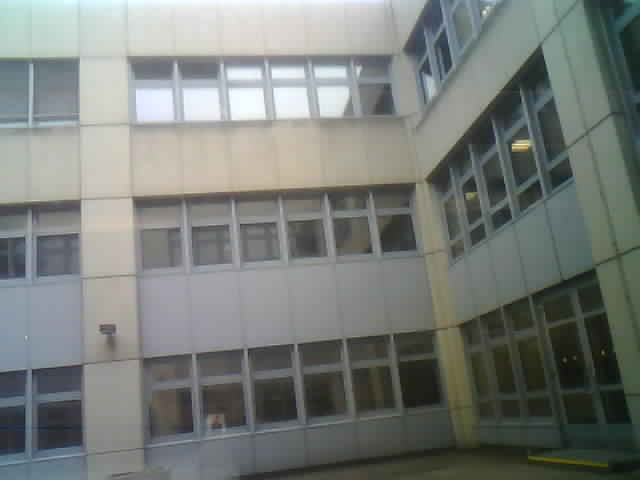
\includegraphics[width=0.7\textwidth, center]{img/cam_erstes_bild.png}
		\caption{Erstes empfangenes Bild der ESP32-CAM}
		\label{cam_erstes_bild}
	\end{figure}
	\subsection{Sensoren}
	\subsubsection{LiDAR}
	\subsubsection{Gyroskop}
	\subsubsection{Encoder}
	\subsubsection{Kompass}
	\section{Backend-Server}
	\subsection{Datenverwaltung}
	\subsection{Roboterpositionen}
	\section{Web-Interface}
	\subsection{LiDAR-Karte}
	\subsection{Anzeigen der Sensordaten}
	\subsection{Fernüberwachung per Kamera}

	% Abbildungs- und Tabellenverzeichnis
	\newpage
	\pagenumbering{gobble}
	\begin{appendix}
		\addcontentsline{toc}{section}{Abbildungsverzeichnis}
		\listoffigures
		\addcontentsline{toc}{section}{Tabellenverzeichnis}
		\listoftables
	\end{appendix}
	\vspace{1cm}
\end{document}